\chapter{Objetivos}

Cuando se empieza a desarrollar una aplicación se suelen cometer muchos errores que ralentizan el periodo de aprendizaje. Para intentar perder el menor tiempo posible es recomendable seguir ciertos pasos:

\section{Familiarizarse con el lenguaje}
Lo primero que debemos hacer antes de empezar a desarrollar nada, es relacionarnos con el lenguaje, en nuestro caso es bastante sencillo porque solo necesitamos manejar javascript para desarrollar la aplicación entera. Lo suyo es empezar haciendo pequeñas funcionalidades en javascript para quitarnos el miedo de encima. Recomiendo hacer pequeños programas que nos ayude a entender las particularidades de javascript.


\section{Como funciona M.E.A.N.}

Una vez que manejamos javascript con bastante soltura, podemos empezar a entender como funciona nuestros stack.

\begin{figure}[H]
    \centering
    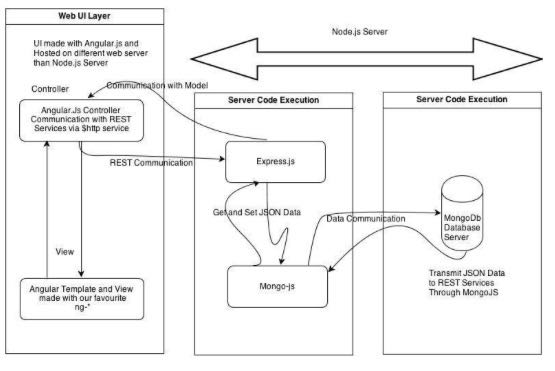
\includegraphics[width=100mm]{meandiag.jpeg}
\end{figure}

En este diagrama podemos apreciar el diagrama de bloque del stack MEAN, en el distinguimos tres grandes bloques:

\begin{itemize}

    \item Web UI Layer: Este bloque hace referencia a la interfaz de usuario, o lo que podemos entender como el cliente(frontend) desarrolado en su totalidad por el framework Angular 2. Esta parte del stack es el que le llega a los usuarios, forma una parte esencial en la aplicación ya que es en todo sus efectos la cara visible de la aplicación.

    
    \item Server Code Execution : Este segundo bloque hace referencia al servidor encargado de atender a cualquier petición del cliente. Este bloque es vital para la inteligencia de la aplicación ya que es el encargado de hacer de intermediario entre el cliente y la base de datos. 


    \item Database Server: Por último destacamos el bloque perteneciente a la base de datos, sin ella no podriamos tener una amplia lista de alumnos y profesores. 

 
\end{itemize}

\section{Pasos para desarrollar una app MEAN}

Una vez que tengamos una buena soltura con javascript y entendamos el funcionamiento del stack MEAN, podemos empezar a meternos en materia.

\begin{itemize}

\item1. Lo primero sería tener montado un "Hola Mundo" en MEAN, para tener organizada nuestro directorio y hacer modificaciones desde ahí.

\item2. Una vez tengamos nuestra aplicación web organizada, es típico error comenzar con la parte del cliente ya que parece una parte más vistosa y por lo tanto más amena. La apariencia de la app debe ser lo que menos te debe importar en este momento. Lo suyo es empezar por el desarrollo del back-end, aportandole la inteligencia necesaría para que con un cliente artificial, llamado postman podamos hacer pruebas de su funcionamiento.

\item3. Una vez tengamos un backend solido y consistente, empezamos con la implementación de controladores y modelos para la gestión de la base de datos. Esto permite que el backend pueda hacer cualquier petición a la base de datos y devolver el resultado a cliente. Volveremos hacer pruebas con Postman nuestro cliente artificial que nos permite saber si nuestro backend esta funcionando correctamente.

\item4. Por último y cuando estemos seguros de que nuestro backend y nuestra base de datos funcionan correctamente, empezaremos a desarrollar nuestra interfaz de usuario. Digamos que es la parte más bonita del desarrollo de una aplicación, debido a que los cambios en código suelen tener un cambio visual que hace que la programación sea más entretenida. 

\end{itemize}